\documentclass{beamer}

\usepackage{listings}
% Copyright 2017 Sergei Tikhomirov, MIT License
% https://github.com/s-tikhomirov/solidity-latex-highlighting/

\usepackage{listings, xcolor}

\definecolor{verylightgray}{rgb}{.97,.97,.97}

\lstdefinelanguage{Solidity}{
	keywords=[1]{anonymous, assembly, assert, balance, break, call, callcode, case, catch, class, constant, continue, constructor, contract, debugger, default, delegatecall, delete, do, else, emit, event, experimental, export, external, false, finally, for, function, gas, if, implements, import, in, indexed, instanceof, interface, internal, is, length, library, log0, log1, log2, log3, log4, memory, modifier, new, payable, pragma, private, protected, public, pure, push, require, return, returns, revert, selfdestruct, send, solidity, storage, struct, suicide, super, switch, then, this, throw, transfer, true, try, typeof, using, value, view, while, with, addmod, ecrecover, keccak256, mulmod, ripemd160, sha256, sha3}, % generic keywords including crypto operations
	keywordstyle=[1]\color{blue}\bfseries,
	keywords=[2]{address, bool, byte, bytes, bytes1, bytes2, bytes3, bytes4, bytes5, bytes6, bytes7, bytes8, bytes9, bytes10, bytes11, bytes12, bytes13, bytes14, bytes15, bytes16, bytes17, bytes18, bytes19, bytes20, bytes21, bytes22, bytes23, bytes24, bytes25, bytes26, bytes27, bytes28, bytes29, bytes30, bytes31, bytes32, enum, int, int8, int16, int24, int32, int40, int48, int56, int64, int72, int80, int88, int96, int104, int112, int120, int128, int136, int144, int152, int160, int168, int176, int184, int192, int200, int208, int216, int224, int232, int240, int248, int256, mapping, string, uint, uint8, uint16, uint24, uint32, uint40, uint48, uint56, uint64, uint72, uint80, uint88, uint96, uint104, uint112, uint120, uint128, uint136, uint144, uint152, uint160, uint168, uint176, uint184, uint192, uint200, uint208, uint216, uint224, uint232, uint240, uint248, uint256, var, void, ether, finney, szabo, wei, days, hours, minutes, seconds, weeks, years},	% types; money and time units
	keywordstyle=[2]\color{teal}\bfseries,
	keywords=[3]{block, blockhash, coinbase, difficulty, gaslimit, number, timestamp, msg, data, gas, sender, sig, value, now, tx, gasprice, origin},	% environment variables
	keywordstyle=[3]\color{violet}\bfseries,
	identifierstyle=\color{black},
	sensitive=false,
	comment=[l]{//},
	morecomment=[s]{/*}{*/},
	commentstyle=\color{gray}\ttfamily,
	stringstyle=\color{red}\ttfamily,
	morestring=[b]',
	morestring=[b]"
}

\lstset{
  language=Solidity,
  escapeinside={<@}{@>},
	backgroundcolor=\color{verylightgray},
	extendedchars=true,
	basicstyle=\footnotesize\ttfamily,
	showstringspaces=false,
	showspaces=false,
	numbers=left,
	numberstyle=\footnotesize,
	numbersep=9pt,
	tabsize=2,
	breaklines=true,
	showtabs=false,
	captionpos=b
}


\usecolortheme{beaver}

\AtBeginSection
{
  \begin{frame}
    \frametitle{Table of Contents}
    \tableofcontents[currentsection]
  \end{frame}
}

\setbeamertemplate{itemize items}{\textbullet}
\setbeamertemplate{footline}[text line]{%
  \parbox{\linewidth}{\vspace*{-8pt}
    \insertshorttitle\hfill\insertshortauthor\hfill\insertframenumber
  }
}
\setbeamertemplate{navigation symbols}{}

\begin{document}

\title{Formal Verification in Scala}
% \subtitle{The Decentralized Autonomous Organization}
\author{Ramon Boss, Anna Doukmak}

\frame{\titlepage}

\begin{frame}
  \frametitle{Table of Contents}
  \tableofcontents
\end{frame}

%%%%%%%%%%%%%%%%%%%%%%%%%%%%%%%%%%%%%%%%%%%%%%%%%%%%%%%%%%%%%%%%%%%%%%%%%%%%%%%%
\section{Formal verification components //TODO: or concept}
%%%%%%%%%%%%%%%%%%%%%%%%%%%%%%%%%%%%%%%%%%%%%%%%%%%%%%%%%%%%%%%%%%%%%%%%%%%%%%%%

\begin{frame}
\frametitle{Stainless}
%\begin{columns}
%  \begin{column}{0.5\textwidth}
  %Basics
  \begin{itemize}
    \item Pure Scala code
    \item Imperative features
    \item Formal specification with pre- and postcondition
    \item Outcomes of verification: valid, invalid, unknown
  \end{itemize}
%  \end{column}
  %\pause
  %\begin{column}{0.5\textwidth}
  %  Technology
  %  \begin{itemize}
  %    \item An open-source software
  %    \item Written in Solidity
  %    \item Build on Ethereum blockchain
  %  \end{itemize}
  %\end{column}
%\end{columns}
\end{frame}


\begin{frame}
\frametitle{Properties to verify}
\begin{itemize}
  \item Bitcoin-S project
  \item No Inflation Property
  \item Addition with Zero Property
\end{itemize}
%\pause
%\begin{lstlisting}[language=Solidity]
%contract DAO is DAOInterface {
%  uint constant minProposalDebatePeriod = 2 weeks;
%  uint public proposalDeposit;
%  mapping (address => bool) public allowedRecipients;

%  function DAO(uint _proposalDeposit) {
%    proposalDeposit = _proposalDeposit;
%    allowedRecipients[address(this)] = true;
%  }
%}
%\end{lstlisting}
\end{frame}


%%%%%%%%%%%%%%%%%%%%%%%%%%%%%%%%%%%%%%%%%%%%%%%%%%%%%%%%%%%%%%%%%%%%%%%%%%%%%%%%
\section{Process of verification //TODO: change the title}
%%%%%%%%%%%%%%%%%%%%%%%%%%%%%%%%%%%%%%%%%%%%%%%%%%%%%%%%%%%%%%%%%%%%%%%%%%%%%%%%


\begin{frame}[fragile]
\frametitle{Verifying No Inflation Property}
\begin{itemize}
  \item Validation of a transaction with \textit{checkTransaction}
  \item Integration of Stainless
  \item Adjusting the property
  \item Bug in \textit{checkTransaction}
\end{itemize}
\pause
\begin{lstlisting}[language=Scala]
  val prevOutputTxIds = transaction.inputs.map(_.previousOutput.txId)
  val noDuplicateInputs = prevOutputTxIds.distinct.size == prevOutputTxIds.size
\end{lstlisting}
\end{frame}


\begin{frame}
\frametitle{Bugfix}
\centering
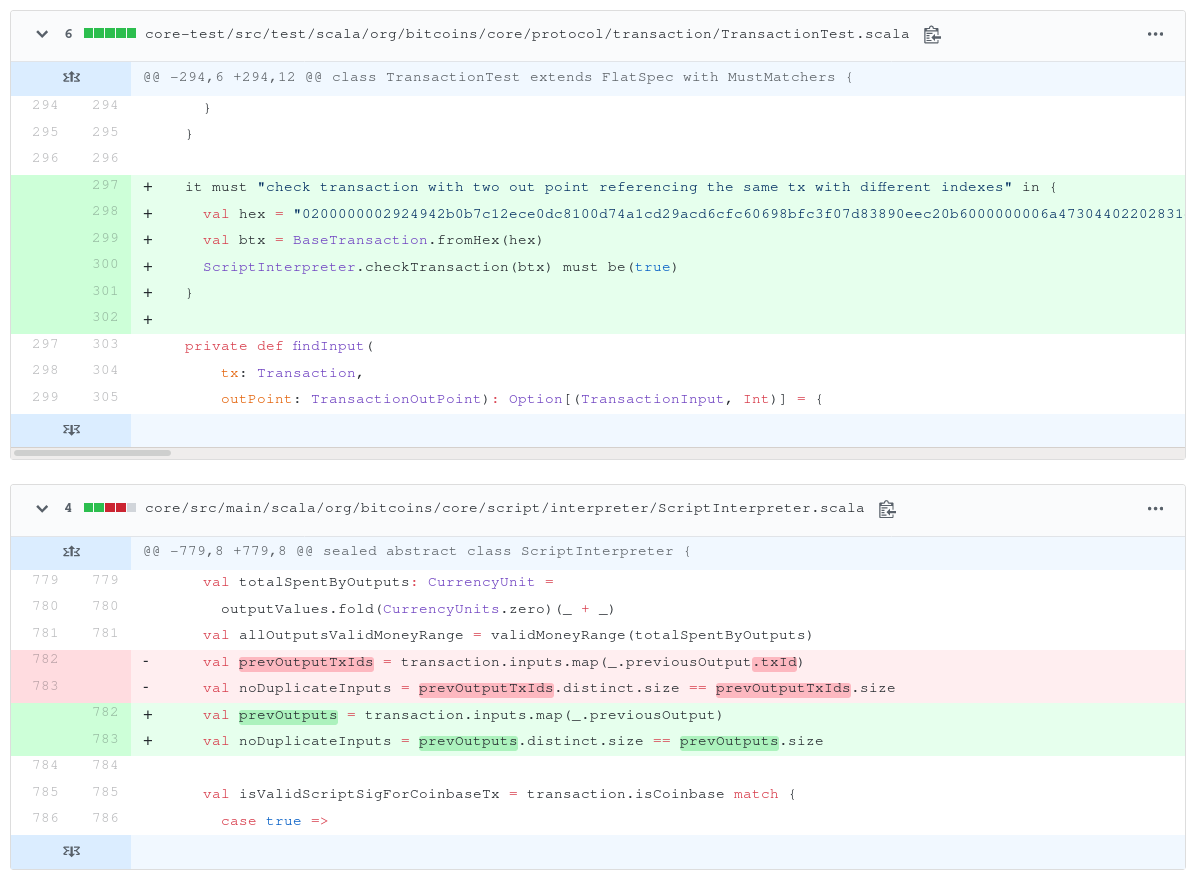
\includegraphics[width=\textwidth,height=0.8\textheight,keepaspectratio]{assets/bitcoin-s-pr.png}
\end{frame}


\begin{frame}[fragile]
\frametitle{Verifying Addition with Zero}
\begin{itemize}%[<1-2>]
  \item Datatype Satoshis
  \item Method for verification
  \begin{lstlisting}[language=Scala, numbers=none]
    +(c: CurrencyUnit): CurrencyUnit
  \end{lstlisting}
  \item Rewriting 2 classes into Pure Scala
\end{itemize}
\end{frame}


\begin{frame}
\frametitle{Rewriting the code}
\end{frame}


\begin{frame}[fragile]
\frametitle{Formal specification}
\begin{lstlisting}[language=Scala]
  override def +(c: CurrencyUnit): CurrencyUnit = {
    require(c.satoshis == Satoshis.zero)
    Satoshis(satoshis.underlying + c.satoshis.underlying)
  } ensuring(res => res.satoshis == this.satoshis)
\end{lstlisting}
\end{frame}


%%%%%%%%%%%%%%%%%%%%%%%%%%%%%%%%%%%%%%%%%%%%%%%%%%%%%%%%%%%%%%%%%%%%%%%%%%%%%%%%
\section{Results}
%%%%%%%%%%%%%%%%%%%%%%%%%%%%%%%%%%%%%%%%%%%%%%%%%%%%%%%%%%%%%%%%%%%%%%%%%%%%%%%%

\begin{frame}
\frametitle{Output of Stainless}
\centering
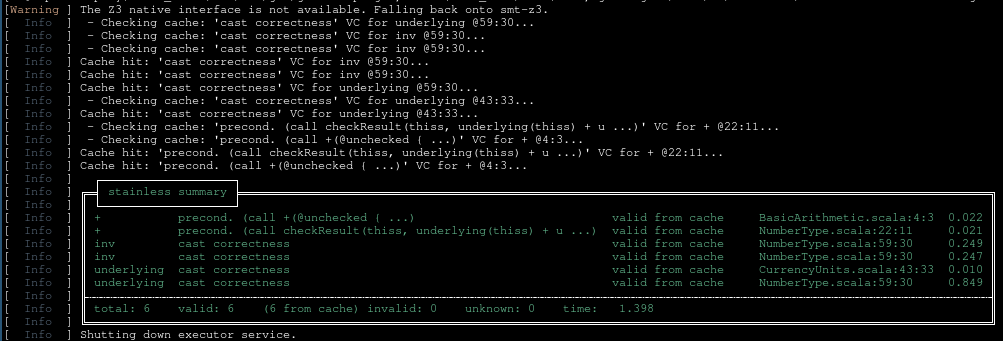
\includegraphics[width=\textwidth,height=0.8\textheight,keepaspectratio]{assets/final_verify_output.png}
\end{frame}


\end{document}
